\large{
È stato realizzato il primo editor in grado di lavorare su grafi definibili "\textit{multilivello}". Questa realizzazione reca un grande aiuto nell'automazione della visualizzazione di grafi e della loro struttura. Potendo visualizzare le strutture si potrà velocizzare la ricerca e la risoluzione di problemi che risultano essere di grande interesse nella teoria dei grafi e dell'informatica teorica.\\
La riduzione polinomiale riportata presenta inoltre un traguardo della ricerca che permette di eseguire indagini sulla complessità della planarità di un grafo clusterizzato legittimamente limitate a grafici flat di grafi planari(indipendenti), trascurando gerarchie più complesse dell'albero di inclusione.\\
Essendo un editor realizzato come progetto finale di un percorso di tesi di laurea potranno essere inoltre realizzati degli sviluppi futuri riportati di sequito.
Un possibile sviluppo futuro per quanto concerne l'aumento delle possibilità di interazione dell'utente con il sistema si possono prendere due strade:
\begin{itemize}
	\item realizzare nuove operazioni di modifica o di creazione a disposizione dell'utente;
	\item aumentare il grado di interazione passando da un grado di livello $0$ ad un grado di livello $3$ per quanto riguarda la rappresentazione della struttura dati nella TreeView consentendo all'utente di avere interazioni di trasformazione anche in quella visualizzazione.
\end{itemize}

Per quanto riguarda invece le modalità di creazione di una istanza equivalente mediante riduzioni polinomiali.
A tal proposito, sempre nell'ambito del problema del decidere quanto un grafo clusterizzato ammette un disegno c-planare, è possibile la realizzazione anche della riduzione in disegno planare Pipe che sarà introdotta di seguito e la cui composizione, partendo da un disegno planare Flat fino alla costruzione del disegno c-planare Pipe, è mostrata nella  \figurename~\ref{fig:composizionePipe}.
\begin{figure}[!htb]
	\begin{center}
		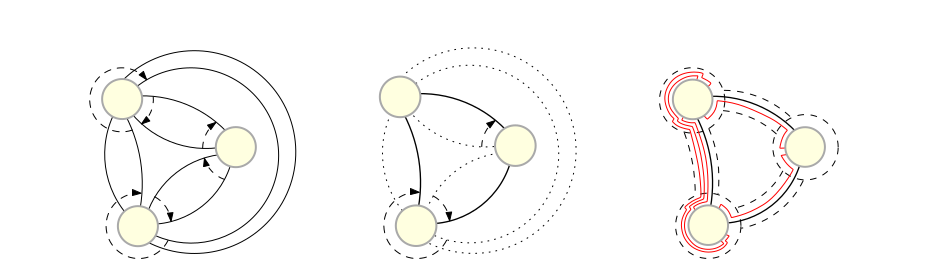
\includegraphics[width=1 \linewidth]{figure/composizionePipe}
	\end{center}
	\caption{creazione di un disegno c-planare Pipe partendo da un disegno c-planare Flat \label{fig:composizionePipe}}
\end{figure}
Avendo già definito i concetti di grafo clusterizzato, disegno planare, riduzione polinomiale e tutto ciò che ne concerne definiamo adesso il concetto di pipe su cui si basa la riduzione.
Sia $\Gamma(C)$ un disegno c-planare di un c-grafico $C$. Per ogni cluster $\mu_i$ di $C$, il disegno $\Gamma$ induce un ordine $O_{orario}(\mu_i)$ in senso orario dei bordi tra cluster di $\mu_i$, ovvero l'ordine circolare in cui si incontrano i bordi tra i cluster di $\mu_i$ mentre si attraversa in senso orario il limite di $R(\mu_i)$ in $\Gamma$. Allo stesso modo, definiamo l'ordinamento antiorario $O_{antiorario}(\mu_i)$ dei bordi tra cluster di $\mu_i$. Un disegno c-planare Pipe $\Gamma_p(C)$ di un grafo flat $C(G, T)$ è un disegno c-planare di $C$ tale che, per qualsiasi coppia di cluster vicini $\mu_i$ e $\mu_j$, esiste un semplice regione chiusa $R(\mu_i, \mu_j)$, detta Pipe, che tocca $R(\mu_i)$ e $R(\mu_j)$ e che contiene esclusivamente la porzione dei bordi inter-cluster in $E(\mu_i, \mu_j)$ all'esterno di $R(\mu_i)$ e $R(\mu_j)$.\\

\begin{figure}[!htb]
	\begin{center}
		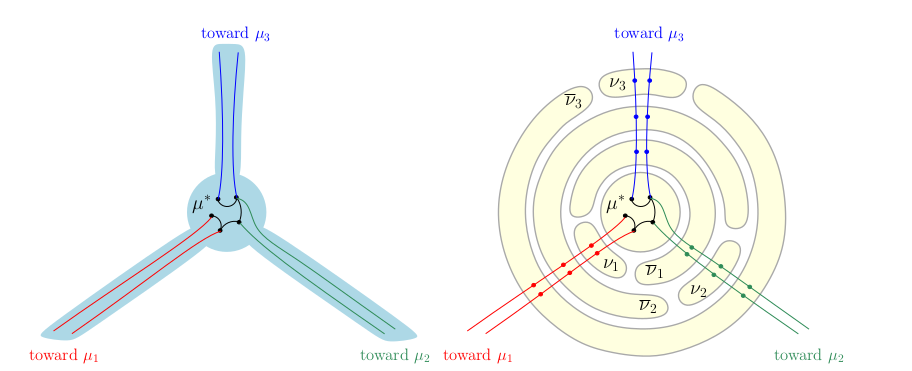
\includegraphics[width=1 \linewidth]{figure/flatVsPipe}
	\end{center}
	\caption{Dettaglio di un cluster in c-planare Pipe ed in c-planare Flat \label{fig:flatVsPipe}}
\end{figure}

Per concludere la visualizzazione delle informazioni risulta essere un ambito che nel prossimo futuro rivestirà un ruolo importante in quanto si sta assistendo alla grande crescita per quanto riguarda la quantità di dati creati ed elaborati. Essendo poi, nella teoria dei grafi, i problemi riguardanti i grafi clusterizzati ed il disegno planare ambito di studio aperto da venti anni e ben lontano dalla fine delle ricerche, si ritrova di grande valore accademico il sistema realizzato. 
}
